\documentclass[12pt]{article} % 11pt font
% 1in margins
\usepackage[margin=1in]{geometry}
\usepackage{pdfpages}
\usepackage{amsmath}
\usepackage{amsfonts}
\usepackage{amssymb}
\usepackage{graphicx}
\usepackage{listings}
\usepackage{float}
\usepackage{hyperref}
\usepackage{algorithm}
\usepackage{algorithmic}
\usepackage{xcolor}
\usepackage{setspace}
\usepackage[numbers]{natbib}
\usepackage{parskip}
\newcommand{\red}[1]{\textcolor{red}{#1}}
\title{The Lanczos Algorithm in Quantum Chemistry}
\author{Patryk Kozlowski and Hamlin Wu}
\date{\today}
\begin{document}
\maketitle
\section*{Page Zero - 4 Declarations}
\subsection*{Textbook Chapters}
This work is most closely related to chapters 2 and 4 of Heath. 
\subsection*{Contributions of Authors}
P.K. was responsible for the writeup associated with the application of the Lanczos method to moment-conserving $GW$. He also wrote the supporting code for the project. H.W. was responsible for writeup of the general exposition of the Lanczos method.
\subsection*{Use of AI Tools}
One of us used ChatGPT to help with the coding elements.
\subsection*{Other Sources}
No conversations besides those between the authors themselves was had regarding the project.
\clearpage
\section{Introduction}
The Lanczos algorithm is often exploited as a means to obtain a few extremal eigenvalues of large sparse Hermitian matrices. It was concieved by the Hungarian mathematician Cornelius Lanczos while working for the U.S. National Bureau of Standards between the years of 1949 and 1952. \cite{golubHistory, Lanczos:1950zz} Since its inception, it has been of considerable value for solving problems in the physical sciences which formally reduce to finding the lowest eigenenergy and eigenvector of a large Hamiltonian matrix.

The core utility the Lanczos algorithm provides is to tridiagonalize large Hermitian matrices iteratively. Before we describe the key mechanisms which enable the Lanczos algorithm, it is worth spending some time considering the merits of the Lanczos algorithm in comparison to other means of tridiagonalizing matrices. As we have seen in class, one means of constructing a tridiagonal matrix is through the use of Householder reflectors. Given a Hermitian matrix $\mathcal{H}$ of dimension $n$, this is to say that we seek a set of $n$ Householder reflectors, which are themselves unitary matrices, satisfying the following, where $T$ is a tridiagonal matrix. 
\begin{equation}
    T = Q^*_n Q^*_{n-1}...Q^*_1 \mathcal{H} Q_1 ... Q_{n-1}Q_n 
\end{equation}
As usual, $^*$ denotes the conjugate transpose of a given matrix.
Pictorially, we may imagine each $Q_n$ zeroing out elements in a given column below a certain row. The ingredients we must prepare in a direct tridiagonalization of a given matrix are thus the Household reflectors $Q_n$, which are to be computed. As the product of unitary matrices is itself unitary, we may re-write the above equation in the following form, where $\textbf{Q} = Q_1 ...  Q_{n-1}Q_n$.
\begin{equation}
    \begin{aligned}
        T &= \textbf{Q}^* \mathcal{H} \textbf{Q}\\
        \mathcal{H} &= \textbf{Q} T \textbf{Q}^*
    \end{aligned}
\end{equation}
One lesson we can take from this last equation is that by choosing a suitable orthonormal basis, which is encoded as the columns of $\textbf{Q}$, we may represent $\mathcal{H}$ in tridiagonal form. The direct algorithm, as we saw in class carries an operation count that scales as $O(n^3)$, though is remarkably stable. This scaling makes the use of such an algorithm impractical when the dimension $n$ of a matrix in consideration is large. An alternative to using Householder reflectors is to use the so called Givens rotation matrices, as described in section 3.5 in Heath, though this generally requires greater computational cost \cite{doi:10.1137/1.9781611975581}. Yet another way of constructing $\textbf{Q}$ is the Gram-Schmidt orthogonalization process, which we saw in class and is described in Heath \cite{doi:10.1137/1.9781611975581}. However as noted in lecture and in Heath, though this method is exact in principle, it may suffer from numerical instabilities due to a loss of orthogonality from accumulated rounding errors and requires the computation of the entire matrix $\textbf{Q}$.   Though this is nowhere close to a complete comparison of the Lanczos algorithm with other tridiagonalization methods, it does show that looking back to the $1950$s, there was a demand for computationally efficient means of obtaining matrices in tridiagonal form, which would then allow for specific eigenvalues to be accessed. The Lanczos algorithm rose to the occasion. 

There are a multitude of intricacies associated with the algorithm, concerning stability and efficiency, among other things. Below, we will focus on an elementary overview of the key aspects of the method, loosely following the presentation in Heath. \cite{doi:10.1137/1.9781611975581}

\subsection{Recurrence Relation}
The direct determination of $\textbf{Q}$, which is a product of $n$ Householder reflections is computationally costly. We shall first analyze the structure of the product in equation 1, which will lead to the central recurrence relation of the Lanczos algorithm.

We begin by considering the product of $\mathcal{H}$ with a truncated version of $\textbf{Q}$, which is defined by restricting the original matrix to its first $m$ columns.
\begin{equation}
    \textbf{Q}_m := [q_1 q_2 ... q_m]
\end{equation}
In the above, $q_i$ represent the $i$th column of  $\textbf{Q}$. It may be worthwhile to switch gears for a moment and consider from another perspective where $\textbf{Q}$ arises. To do so, we introduce the notion of a Krylov matrix, $\mathcal{K}_n$, given a matrix $\mathcal{H}$ and an arbitrary (non-zero) vector $v$.
\begin{equation}
    \mathcal{K}_n := [v \enspace \mathcal{H}v\enspace \mathcal{H}^2v ... \enspace \mathcal{H}^{n-1} v]
\end{equation}
The space spanned by this matrix is termed the Krylov subspace. Applying the matrix $\mathcal{H}$ to $\mathcal{K}_n$, we have
\begin{equation}
    \mathcal{H}\mathcal{K}_n = [\mathcal{H}v \enspace \mathcal{H}^2v \enspace ... \mathcal{H}^n v] = \mathcal{K}_n[\textbf{e}_2 \enspace \textbf{e}_3 ... \mathcal{K}_n^{-1} \mathcal{H}^n v]
\end{equation}
Here, $\textbf{e}_i$ represents a column vector with only a one in the $i$th row. Based on the structure of the latter matrix in equation 5, it is necessarily upper Hessenberg, and is termed $C_n$ in Heath. This implies that we may write $\mathcal{H}$ as the following.
\begin{equation}
    \mathcal{H} = \mathcal{K}_n C_n \mathcal{K}_n^{-1}
\end{equation}
Conducting a QR factorization on $\mathcal{K}_n$, we obtain unitary $Q$ and upper triangular $R$ such that $\mathcal{K}_n = QR$. We then have
\begin{equation}
    \mathcal{H} = QR C_n R^{-1}Q^{-1} 
\end{equation}
which upon using the fact that $Q^{-1} = Q^*$, yields the following.
\begin{equation}
    Q^*\mathcal{H} Q = R C_n R^{-1}
\end{equation}
The similarity transform in the right hand side of equation 8 preserves the upper Hessenberg structure of $C_n$, which implies that the right hand side is additionally tridiagonal due to the Hermiticity of the left hand side. Here, we have shown from another perspective why we have the relation $\mathcal{H} = \textbf{Q} T \textbf{Q}^*$ when $\mathcal{H}$ is a Hermitian matrix. Furthermore, we have learned from this brief excursion that the $\textbf{Q}$ we seek provides an orthonormal basis for the Krylov subspace spanned by $\mathcal{K}_n$

Returning now to our analysis of the product $\mathcal{H}\textbf{Q}_m = \textbf{Q} T \textbf{Q}^* \textbf{Q}_m $, we first analyze the term $\textbf{Q}^*\textbf{Q}_m$. As the columns of $\textbf{Q}$ form an orthonormal basis, the product results in the following.
\begin{equation}
    \textbf{Q}^* \textbf{Q}_m = \begin{bmatrix}
\begin{array}{cccc}
1 & 0 & 0 & \ldots \\
0 & 1 & 0 & \ldots \\
0 & 0 & 1 &\ldots \\
.. & .. & .. & \ldots
\end{array} \\
\hline
\begin{array}{cccc}
0 & 0 & 0 & \ldots\\
0 & 0 & 0 & \ldots\\
..&..&..& \ldots
\end{array}
\end{bmatrix}
\end{equation}
The first $m \times m$ section of this $n\times m$ matrix is an identity block, while the remaining portion of the matrix is zero due to the orthogonal property of the column vectors of $\textbf{Q}$. Now, considering the product of this matrix with $T$, we arrive at the following.
\begin{equation}
    T\textbf{Q}^* \textbf{Q}_m = \begin{bmatrix}
        \begin{array}{cccc}
        \alpha_1 &\beta_1& 0 &...\\
        \beta_1^* & \alpha_2 & \beta_2 & \ldots \\
        0 &\beta_2^* & \alpha_3 & \ldots\\ 
        .. & .. & .. & ..
        \end{array}
    \end{bmatrix}
    \begin{bmatrix}
        \begin{array}{ccc}
1 & 0 & 0 \\
0 & 1 & 0 \\
0 & 0 & 1 \\
.. & .. & ..
\end{array} \\
\hline
\begin{array}{ccc}
0 & 0 & 0 \\
0 & 0 & 0 \\
..&..&..
\end{array}
    \end{bmatrix}
\end{equation}
Consider an arbitrary element of this product, noting that we may truncate the sum representing each matrix element at index $m$, which is the row after which the product matrix $\textbf{Q}^* \textbf{Q}_m$ is zero.
\begin{equation}
    (T\textbf{Q}^* \textbf{Q}_m)_{ab} = \sum_j T_{aj} (\textbf{Q}^*\textbf{Q}_m)_{jb} = \sum_{j=1}^m T_{aj} (\textbf{Q}^*\textbf{Q}_m)_{jb} 
\end{equation}
Due to the fact that $(\textbf{Q}^* \textbf{Q}_m)_{jb}$ is just representative of the identity matrix when $j \leq m$, the above matrix element for $a,b \leq m$ are simply the analogous matrix elements of $T$. The one extra matrix element occurs when we consider $a = m+1$, for which the matrix element will simply yield $\beta_m^*$, which is the only entry of $T$ aligning with the lower right one in the product matrix $\textbf{Q}^*\textbf{Q}_m$. This yields the following matrix.
\begin{equation}
(T \textbf{Q}^* \textbf{Q}_m)_{ab} = \begin{bmatrix}
\begin{array}{cccc}
\alpha_1 & \beta_1 & 0 & \cdots \\
\beta_1^* & \alpha_2 & \beta_2 & \cdots \\
\vdots & \ddots & \ddots & \ddots \\
0 & \cdots & \beta_{m-1}^* &\alpha_ m \\
\end{array}\\
\hline
\begin{array}{cccc}
0 \enspace \enspace \enspace& .. &.. & \enspace \; \;\beta_m^* \\
\end{array}
\end{bmatrix}
\end{equation}
We need not explicitly evaluate the last matrix product. We first envision writing the above matrix as a sum of the part above the horizontal line, and a matrix with one element $\beta_m^*$. In equation form, this is given by the following, where we denote $T_m$ to be $T$ restricted to the first $m$ rows and columns and $\textbf{Q}_m$ and $\textbf{e}_m$ as before. 
\begin{equation}
    \mathcal{H}\textbf{Q}_m = \textbf{Q}_m T_m + \beta_{m}^*q_{m+1}\textbf{e}^T_{m}
\end{equation}
Recalling that we are considering $\mathcal{H}\textbf{Q}_m = \textbf{Q} T \textbf{Q}^* \textbf{Q}_m$, we consider the $m$th column of the resulting matrix on each side. On the left, the $m$th column is simply given by the product $\mathcal{H}q_m$ where $q_m$ is the $m$th column of $\textbf{Q}_m$. On the right hand side, the first contribution to the $m$th column will come from the product of $\textbf{Q}$ and the portion of the matrix above the line, which will yield $q_m \alpha_m + q_{m-1} \beta_{m-1}$. The second contribution comes from the portion of the matrix below the horizontal line, and will be of the form $q_{m+1}\beta^*_m$. We thus arrive at the recurrence equation below, which tells us how to iteratively build the columns of \textbf{Q}.
\begin{equation}
    \mathcal{H} q_m = q_m \alpha_m + q_{m-1} \beta_{m-1} + q_{m+1}\beta^*_m
\end{equation}
\begin{equation}
    q_{m+1} = \frac{1}{\beta^*_m}(q_m \alpha_m + q_{m-1}\beta_{m-1} - \mathcal{H}q_m)
\end{equation}
We may now define the Lanczos iteration, which is the central component of the Lanczos algorithm.
\subsection{Lanczos iteration}
Using the three-term recursion relationship which we have previously described, we may formally spell out what the Lanczos iteration does. Starting with initial values $\beta_0 = 0$ and $q_0 = 0$ and an initial normalized random vector $q_1$, we may proceed to generate subsequent columns using equation 15. We additionally make the note that due to the orthogonality of the columns of $\textbf{Q}$, we may obtain $\alpha_m$ by projecting equation 14 by $q^*_m$.
\begin{algorithm}
    \caption{Lanczos iteration}
    \begin{algorithmic}[1]
    \REQUIRE Hermitian matrix $\mathcal{H}$ of dim $n$, normalized vector $v$
    \STATE $\beta_0 = 0$
    \STATE $q_0 = \textbf{0}$
    \STATE $q_1$ = $v$
    \FOR{$i = 1$ to $n$}
        \STATE $x_i = \mathcal{H}q_{i}$
        \STATE $\alpha_i = q_{i}^* x_i$
        \STATE $q_{i+1} = q_i \alpha_i + q_{i-1}\beta_{i-1} - x_i$ 
        \STATE $\beta_i = ||q_{i+1}||_2$
        \STATE $q_{i+1} = q_{i+1}/ \beta_i$
    \ENDFOR
    \end{algorithmic}
\end{algorithm}
From the shown algorithm, we see that should we come across an iteration where $\beta_i = 0$, we must stop else we divide by zero. This would signal a decoupling of the matrix $T$, meaning that we have stumbled upon an invariant subspace which we may then examine. A key feature of the Lanczos algorithm is that we need not build up the entire matrix $\textbf{Q}$, and can arrive at a sufficiently good approximation of $T$ within a reasonable number of iterations, allowing for select extremal eigenvalues to be determined by other means. In the attached code, we have implemented this Lanczos iteration, and have used it to compute the extremal eigenvalues of the Hamiltonian matrix. As can be seen in the first appended figure, Lanczos is able to obtain a good approximation of the lowest eigenvalues of a Hermitian matrix already in the first few iterations; as more iterations are used, one also obtains better estimates of the higher values, but at the expense of a higher cost.
\subsection{Ritz Values and Extremal Eigenvalues}
As mentioned in Parlett's textbook, round-off errors which result in non-orthogonality between the determined $q_i$ may hinder the efficacy of the Lanczos method without further modifications improving the robustness of the method. \cite{Parlett} As mentioned within Chapter 13 of Parlett's book, yet another perpsective from which the Lanczos algorithm may be viewed is through the lens of the Rayleigh-Ritz method.

We begin by returning briefly to Krylov subspaces. The power method is the basic method of computing extremal eigenvalues and eigenvectors, with the main idea that with repeated application of a matrix $\mathcal{H}$ to a vector $v$, eventually the component corresponding to the eigenvector with largest eigenvalue will dominate. By the definition of the power method, consecutive iterations of the algorithm will produce an increasing sequence of Krylov subspaces. In equations, this is to say that after the $n$th power iteration on some starting vector $v$, we produce a Krylov subspace spanned by the following Krylov matrix.
\begin{equation}
    \mathcal{K}_{n+1} = [v \enspace \mathcal{H}v \enspace \mathcal{H}^2 v \enspace ... \enspace \mathcal{H}^{n}v]
\end{equation}
The hope of the power method is that with successive iterations, $\mathcal{H}^n v$ will converge to a vector representing an eigenvector of $\mathcal{H}$ with largest eigenvector. One can imagine that this simple procedure does not yield optimal estimations of the desired eigenvector. The fruitful question of asking instead for the best approximation to the true eigenvector within the space spanned by $\mathcal{K}_{n+1}$ is the basis of the Lanczos algorithm when viewed from the perspective of the Rayleigh-Ritz method. By nature of its construction, the natural basis of a Krylov subspace given by the vectors $\{v, \mathcal{H}v, \mathcal{H}^2v ...\}$ is prone to be ill-conditioned due to linear-dependency errors which may arise from repeated iterations. As we have seen before, the Lanczos algorithm provides a means of iteratively generating an orthonormal basis for Krylov subspaces of increasing dimension. If we consider a normalized eigenvector and eigenvalue of $T_m$ as defined in equation 13 satisfying $T_m \phi = E \phi$ and consider right projecting equation 13 on the right by the eigenvector, we get the following.
\begin{equation}
    \mathcal{H}\textbf{Q}_m \phi = \textbf{Q}_m T_m \phi + \beta^*_m q_{m+1}e^{T}_m \phi = \textbf{Q}_m E \phi + \beta^*_m q_{m+1}e^{T}_m \phi 
\end{equation}
The approximate eigenvalues of $\mathcal{H}$, $E$, are termed the Ritz values, and we may see that the additional term $\beta^*_m q_{m+1}e^T_m \phi$ provides a measure of how far $\textbf{Q}_m \phi$ differs from being a true eigenvector of $\mathcal{H}$. Tracking the magnitude of this residual term thus provides a metric of how close our approximate eigenvectors, obtained from $T_m$, are to the true eigenvectors we desire. This can be seen from the fact that if the last term was to vanish, then $\textbf{Q}_m \phi$ would be an exact eigenvector of $\mathcal{H}$ with eigenvalue $E$. One can compute the extremal eigenvalues by tracking the evolution and convergence of the extremal Ritz values with each successive iteration.

Thus far, we have touched on some of the fundamentals which power the Lanczos method on a surface level, and have interpreted the algorithm from several perspectives. In the following section, we will describe a form of the Lanczos algorithm which is suitable for the application we consider in section 2.
\subsection{Block Lanczos}
The work of \citet{backhouse2023dynamics} involves the use of a block Lanczos procedure, a generalization of the previously described Lanczos iteration, and we will describe it here. For initialization of the iteration, now instead of a single vector $\mathbf{q}$ we will start with a block vector $\textbf{Q}\equiv [\mathbf{q}_1, \mathbf{q}_2, ... , \mathbf{q}_b]$. Note that the components of this block vector must be orthonormal column vectors, which we enforce with a QR decomposition in the code. The resulting Krylov subspace will therefore be defined as $\mathcal{K}_i(\textbf{H}, \textbf{Q}_1) = \text{span}\{\textbf{Q}_1, \mathbf{H}\textbf{Q}_1, \mathbf{H}^2\textbf{Q}_1,\ldots, \mathbf{H}^{i-1}\textbf{Q}_1\}$; successive $i-1$ applications of the Hamiltonian matrix onto the block vector $\textbf{Q}_1$ form the Krylov subspace. The projection of the Hamiltonian $\textbf{H}$ onto this subspace now gives a \emph{block} tridiagonal form. The algorithm to achieve this goal works as follows:
\begin{align}
\mathbf{R}_i & =\mathbf{H} \mathbf{Q}_i \label{eq:block_lanczos_R1} \\
\mathbf{A}_i & =\mathbf{Q}_i^{\dagger} \mathbf{R}_i \label{eq:block_lanczos_A} \\
\mathbf{R}_i & =\mathbf{R}_i-\mathbf{Q}_i \mathbf{A}_i-\mathbf{Q}_{i-1} \mathbf{B}_{i-1} \label{eq:block_lanczos_R2} \\
\mathbf{Q}_{i+1} \mathbf{B}_i^{\dagger} & =\mathbf{R}_i. \label{eq:block_lanczos_Q}
\end{align}
Qualitatively, we can understand this iteration as follows. Starting with an initial block vector $\mathbf{Q}_i$ taken from the tail end of the Krylov subspace, equation \ref{eq:block_lanczos_R1} projects the $\mathbf{H}$ onto the $\mathbf{Q}_i$. This is our first attempt at forming something ``new''. Next, we produce $\mathbf{A}_i$, by multiplying the current block vector $\mathbf{Q}_i$ with the current residual vector $\mathbf{R}_i$. We store the result, because eventually a string of these $\mathbf{A}_i$ will go on to form the diagonal of the tridiagonal matrix we seek. Then, we refine our residual $\mathbf{R}_i$ by subtracting from it the product of the current $\mathbf{A}_i$ with $\mathbf{Q}_i$ as well as the previous $\mathbf{B}_{i-1}$ with $\mathbf{Q}_{i-1}$. In the last step of the iteration, we obtain $\mathbf{B}_i$ and the next addition to the Krylov subspace $\mathbf{Q}_{i+1}$ by performing a QR decomposition of the current residual vector $\mathbf{R}_i$ in equation \ref{eq:block_lanczos_Q}. This can be understood as a way to combine the final two steps of the Lanczos iteration for simple vectors, which are obtaining the 1) off-diagonal $\beta_i =\left\|\mathbf{r}_i\right\|$ via normalization of the residual and 2) subsequent Lanczos vector $\mathbf{q}_{i+1} =\mathbf{r}_i / \beta_i$ by division of the residual with the off-diagonal $\beta$ we just obtained; via QR factorization we perform both steps in one fell swoop. In the end, block Lanczos can be summarized by the three-term recurrence:
\begin{equation}
 \mathbf{M Q}_i=\mathbf{Q}_{i-1} \mathbf{B}_{i-1}+\mathbf{Q}_i \mathbf{A}_i+\mathbf{Q}_{i+1} \mathbf{B}_i^{\dagger}.
\end{equation}
Block Lanczos can be naively implemented by using recursive function calls, but this is not computationally efficient, so in my appended code, I store the quantities obtained in the given iteration in an array; when I am done I place these in the tridiagonal form:
\begin{equation}
\mathbf{H}_{\text{tri}} = \left[\begin{array}{ccccc}
\mathbf{A}_1 & \mathbf{B}_1 & & & \mathbf{0} \\
\mathbf{B}_1^{\dagger} & \mathbf{A}_2 & \mathbf{B}_2 & & \\
& \mathbf{B}_2^{\dagger} & \mathbf{A}_3 & \ddots & \\
& & \ddots & \ddots & \mathbf{B}_{i-1} \\
\mathbf{0} & & & \mathbf{B}_{i-1}^{\dagger} & \mathbf{A}_i
\end{array}\right].
\end{equation}
It takes less work to find the extreme eigenvalues of a tridiagonal matrix than a general Hermitian matrix. Because this is \emph{block} Lanczos, notice how we are able to accurately compute the 4 lowest eigenvalues at a given time; this corresponds to the fact that in the code I set the block size equal to 4. Similarly to the simple Lanczos, one is only able to get good accuracy for all eigenvalues for a large number of iterations, at which point the computational savings of Lanczos are lost. In quantum chemistry, computing the lowest eigenvalues is usually all that we are interested in because these correspond to the ground state and low lying excited states. To summarize, the idea was to achieve block tridiagonalization via successively building up a Krylov subspace from a block Hermitian matrix and we have implemented this via block Lanczos iteration.
\section{Application in Moment-Conserving $GW$}
\subsection{Motivation}
In the ${GW}$ approximation, one solves for the interacting Green's function $\mathbf{G}$ via the Dyson equation, which is related to the non-interacting Green's function $\mathbf{G}_0$ and the self-energy $\mathbf{\Sigma}$, as $\mathbf{G}=\mathbf{G}_0+\mathbf{G}_0\mathbf{\Sigma}\mathbf{G}=\left[\mathbf{G}_0^{-1}-\mathbf{\Sigma}\right]^{-1}$. Since $\mathbf{G}_0$ is known from a prior mean-field calculation, we are left to determine the self-energy $\mathbf{\Sigma}$. In frequency space, the self-energy can be further broken up as $\mathbf{\Sigma}(\omega)=\mathbf{\Sigma}_{\infty}+\mathbf{\Sigma}^{\text{corr}}(\omega)$, where $\mathbf{\Sigma}_{\infty}$ and $\mathbf{\Sigma}^{\text{corr}}(\omega)$ are the static and dynamic components of the self-energy, respectively. Classically, $\mathbf{\Sigma}^{\text{corr}}(\omega)$ is determined as the convolution of the non-interacting Green's function $\mathbf{G}_0$ with the screened Coulomb interaction $\mathbf{W}$. However, this formulation becomes problematic in frequency space where both $\mathbf{G}_0$ and $\mathbf{W}$ have multiple poles. Therefore, to determine $\mathbf{\Sigma}^{\text{corr}}(\omega)$ we must perform the integral $\mathbf{\Sigma}^{\text{corr}}(\omega)=\int d\omega' e^{i\eta \omega'} \mathbf{G}_0(\omega + \omega')\mathbf{W}(\omega')$, where since the integrand has a complicated pole structure, we introduce the exponential factor $e^{i\eta \omega'}$ and evaluate the resulting contour integral using Cauchy's residue theorem. However, having to evaluate these residues forces one into an unfavorable computational scaling of $\mathcal{O}(N^6)$, where $N$ is the system size. Equivalently, one can formulate this as a matrix problem 
\begin{equation}
    {\mathbf{H}}=\left[\begin{array}{cc}
\mathbf{f}+\boldsymbol{\Sigma}_{\infty} & {\mathbf{W}} \\
{\mathbf{W}}^{\dagger} & {\mathbf{d}}
\end{array}\right],
\end{equation}
If one can diagonalize this Hamiltonian, the rewards are plentiful; the eigenvalues are the charged excitation energies, while the eigenvectors are the quasiparticle Dyson orbitals. However, the matrix $\tilde{\mathbf{H}}$ is large, coupling a small physical space in $\mathbf{f}+\Sigma_{\infty}$ with a large auxiliary space in $\tilde{\mathbf{d}}$ through $\tilde{\mathbf{W}}$. In particular, these quantities are defined as
\begin{gather}
\mathbf{W}_{p, k v}=\sum_{i a}(p k \mid i a)\left(X_{i a}^{v}+Y_{i a}^{v}\right),  \\
\mathbf{d}_{k v, l v^{\prime}}=\left(\epsilon_{k}-\Omega_{v}\right) \delta_{k, l} \delta_{v, v^{\prime}}
\end{gather}
where $X_{ia}^v$ , $Y_{ia}^v$ are eigenvectors, and $\Omega _v$ are the eigenvalues from diagonalizing the Casida equation of time dependent density functional theory (TDDFT), a process that admits the aforementioned steep scaling of $O(N^6)$. However, through the introduction of the moment-conserving self-energy moments by \citet{backhouse2023dynamics}, the above Hamiltonian can be cast into a block tridiagonal form, allowing one to target the extremal eigenvalues with block Lanczos iteration.
\subsection{Lanczos Iteration}
The block tridiagonal form can be expressed as:

\begin{align}
\tilde{\mathbf{H}}_{\text {tri }} & =\tilde{\mathbf{q}}^{(j),\dagger}\left[\begin{array}{cc}
\mathbf{f}+\boldsymbol{\Sigma}_{\infty} & \mathbf{W} \\
\mathbf{W}^{\dagger} & \mathbf{d}
\end{array}\right] \tilde{\mathbf{q}}^{(j)} \\
& =\left[\begin{array}{cccccc}
\mathbf{f}+\boldsymbol{\Sigma}_{\infty} & \mathbf{L} & & & & \mathbf{0} \\
\mathbf{L}^{\dagger} & \mathbf{H}_{1} & \mathbf{C}_{1} & & & \\
& \mathbf{C}_{1}^{\dagger} & \mathbf{H}_{2} & \mathbf{C}_{2} & & \\
& & \mathbf{C}_{2}^{\dagger} & \mathbf{H}_{3} & \ddots & \\
& & & \ddots & \ddots & \mathbf{C}_{j-1} \\
\mathbf{0} & & & & \mathbf{C}_{j-1}^{\dagger} & \mathbf{H}_{j}
\end{array}\right]
\label{eq:tridiagonal}
\end{align}
where we define $\tilde{\mathbf{q}}^{(j)}$ as
\begin{equation}
    \tilde{\mathbf{q}}^{(j)}=\left[\begin{array}{cc}
\mathbf{I} & \mathbf{0} \\
\mathbf{0} & \mathbf{q}^{(j)}
\end{array}\right]
\end{equation}
This formulation becomes exact when the level $j$ equals $N$, corresponding to considering the highest moment of the self-energy, i.e. $n$ ranges from $1,\ldots,N$ (this is made precise in section \ref{sec:self_energy_moments}). In practice, however, we always truncate the Krylov subspace to some $j<N$. Note that the tridiagonal form never forces us to compute $\mathbf{W}$ or $\mathbf{d}$, as desired.

\subsubsection{Creation of Krylov Subspace}
Formally, the Krylov subspace of level $j$ is given as $\mathbf{q}^{(j)}=\left[\mathbf{q}_1, \mathbf{q}_2, \cdots, \mathbf{q}_j\right]$, where the projection of the full Hamiltonian onto this subspace gives the tridiagonal form of equation \ref{eq:tridiagonal}. To start building up the subspace, we need to determine $\mathbf{q}_1$ via QR decomposition of the exact $GW$ couplings as $\mathbf{W}^\dag = \mathbf{q}_1 \mathbf{L}^\dag \rightarrow \mathbf{q}_1 = \mathbf{W}^\dag \mathbf{L}^{\dag, -1}$. $\mathbf{L}$ is defined in terms of just the 0th order self-energy moment as $\mathbf{L}^\dag = \left(\boldsymbol{\Sigma}^{(0)}\right)^{\frac{1}{2}}$. We build up the subsequent $q_i$ vectors through a three-term recurrence
\begin{equation}
    \mathbf{q}_{i+1} \mathbf{C}_i^{\dagger}=\left[\mathbf{d} \mathbf{q}_i-\mathbf{q}_{i} \mathbf{H}_i-\mathbf{q}_{i-1} \mathbf{C}_{i-1}\right],
\end{equation}
where the on-diagonal blocks are defined as
\begin{equation}
    \mathbf{H}_i=\mathbf{q}_i^{\dagger} \mathbf{d} \mathbf{q}_i
\end{equation}
Notice that to form the initial vector $\mathbf{q}_1$ we would need $\mathbf{W}^\dag$ and to continue building the subspace, we would need $\mathbf{d}$, so to avoid this, we introduce the self-energy moments.
\subsection{Tridiagonal Quantities}
\subsubsection{Computing Self-Energy Moments}
\label{sec:self_energy_moments}
The moments of the lesser and greater parts of the self-energy have the form
\begin{equation}
\begin{gathered}
\Sigma_{pq}^{(n,<)}=\sum_{ia, jb, k} \sum_{t=0}^n\binom{n}{t}(-1)^t \epsilon_k^{n-t}(pk \mid ia) \eta_{ia, jb}^{(t)}(qk \mid jb), \\
\Sigma_{pq}^{(n,>)}=\sum_{ia, jb, c} \sum_{t=0}^n\binom{n}{t} \epsilon_c^{n-t}(pc \mid ia) \eta_{ia, jb}^{(t)}(qc \mid jb),\\
\end{gathered}
\end{equation}
respectively. The energies $\epsilon$ and integrals $(pq \mid rs)$ are known to us from the prior mean-field calculation, but the density-density moments $\eta^{(t)}$ are not, so we need to compute them. We find them to be defined as
\begin{equation}
\begin{aligned}
\boldsymbol{\eta}^{(m)} 
& =\left[\boldsymbol{\eta}^{(0)}(\mathbf{A}+\mathbf{B})\right]^m \boldsymbol{\eta}^{(0)} ,
\end{aligned}
\end{equation}
with the initial
\begin{equation}
\boldsymbol{\eta}^{(0)}=[(\mathbf{A}-\mathbf{B})(\mathbf{A}+\mathbf{B})]^{\frac{1}{2}}(\mathbf{A}+\mathbf{B})^{-1} 
\end{equation}
where we have $\mathbf{A}$ and $\mathbf{B}$ with components $A_{ia,jb}=\delta_{ij}\delta_{ab}\left(\epsilon_a - \epsilon_i\right)+(ia \mid jb)$ and $B_{ia,jb}=(ia \mid jb)$.
Note that the scaling of the above would be improved by introducing low-rank approximations to the electron repulsion integrals (ERIs) via the Cholesky decomposition or tensor hyper-contraction, which express these 4-index quantities as a sum of two 3- or five 2-index tensors, respectively.
\subsection{Avoiding auxiliary space}
To avoid using the large auxiliary quantities, we introduce an operator which will project onto the block Lanczos space as $\mathbf{S}_{i,j}^{(n)} =\mathbf{q}_i^{\dagger} \mathbf{d}^n \mathbf{q}_j$. But due to the orthogonality of the Krylov subspace, we have $q_i^\dagger q_j = 0$ for $i\neq j$, so $\mathbf{S}_{i,j}^{(n)} = 0$ for $|i-j|>1$. Furthermore, due to Hermiticity, $\mathbf{S}_{i,j}^{(n)} = \mathbf{S}_{j,i}^{(n) \dagger}$. We can start with the initial definition $\mathbf{S}_{1,1}^{(n)} = \mathbf{q}_1^\dagger \mathbf{d}^n \mathbf{q}_1 = \mathbf{L}^{-1} \mathbf{\Sigma}^{(n)} \mathbf{L}^{-1, \dagger}$.

\begin{equation}
\end{equation}
\begin{equation}
\begin{aligned}
\mathbf{S}_{i+1, i}^{(n)}=&\mathbf{q}_{i+1}^{\dagger} \mathbf{d}^n \mathbf{q}_i=\mathbf{C}_i^{-1}\left[\mathbf{S}_{i, i}^{(n+1)}-\mathbf{H}_i \mathbf{S}_{i, i}^{(n)}-\mathbf{C}_{i-1}^{\dagger} \mathbf{S}_{i-1, i}^{(n)}\right]\\
\mathbf{S}_{i+1, i+1}^{(n)}= & \mathbf{q}_{i+1}^{\dagger} \mathbf{d}^n \mathbf{q}_{i+1}
=  \mathbf{C}_i^{-1}\left[\mathbf{S}_{i, i}^{(n+2)}+\mathbf{H}_i \mathbf{S}_{i, i}^{(n)} \mathbf{H}_i+\mathbf{C}_{i-1}^{\dagger} \mathbf{S}_{i-1, i-1}^{(n)} \mathbf{C}_{i-1}\right. \\
& \left.-P\left(\mathbf{S}_{i, i}^{(n+1)} \mathbf{H}_i\right)+P\left(\mathbf{H}_i \mathbf{S}_{i, i-1}^{(n)} \mathbf{C}_{i-1}\right)-P\left(\mathbf{S}_{i, i-1}^{(n+1)} \mathbf{C}_{i-1}\right)\right] \mathbf{C}_i^{-1, \dagger},
\end{aligned}
\end{equation}
and then solving for $\mathbf{C}_i^2$
\begin{equation}
    \mathbf{C}_i^2=\left[\mathbf{S}_{i, i}^{(2)}+\mathbf{H}_i^2+\mathbf{C}_{i-1}^{\dagger} \mathbf{C}_{i-1}-P\left(\mathbf{S}_{i, i}^{(1)} \mathbf{H}_i\right)-P\left(\mathbf{S}_{i, i-1}^{(1)} \mathbf{C}_{i-1}\right)\right]
\end{equation}
and we can also find the on-diagonal $\mathbf{H}$ matrices using
\begin{equation}
\begin{aligned}
\mathbf{H}_i=\mathbf{q}_i^{\dagger} \mathbf{d} \mathbf{q}_i=\mathbf{S}_{i, i}^{(1)} .
\end{aligned}
\end{equation}
Now, we know how to compute every quantity of equation \ref{eq:tridiagonal}.

\bibliographystyle{plainnat}
\bibliography{citations.bib}
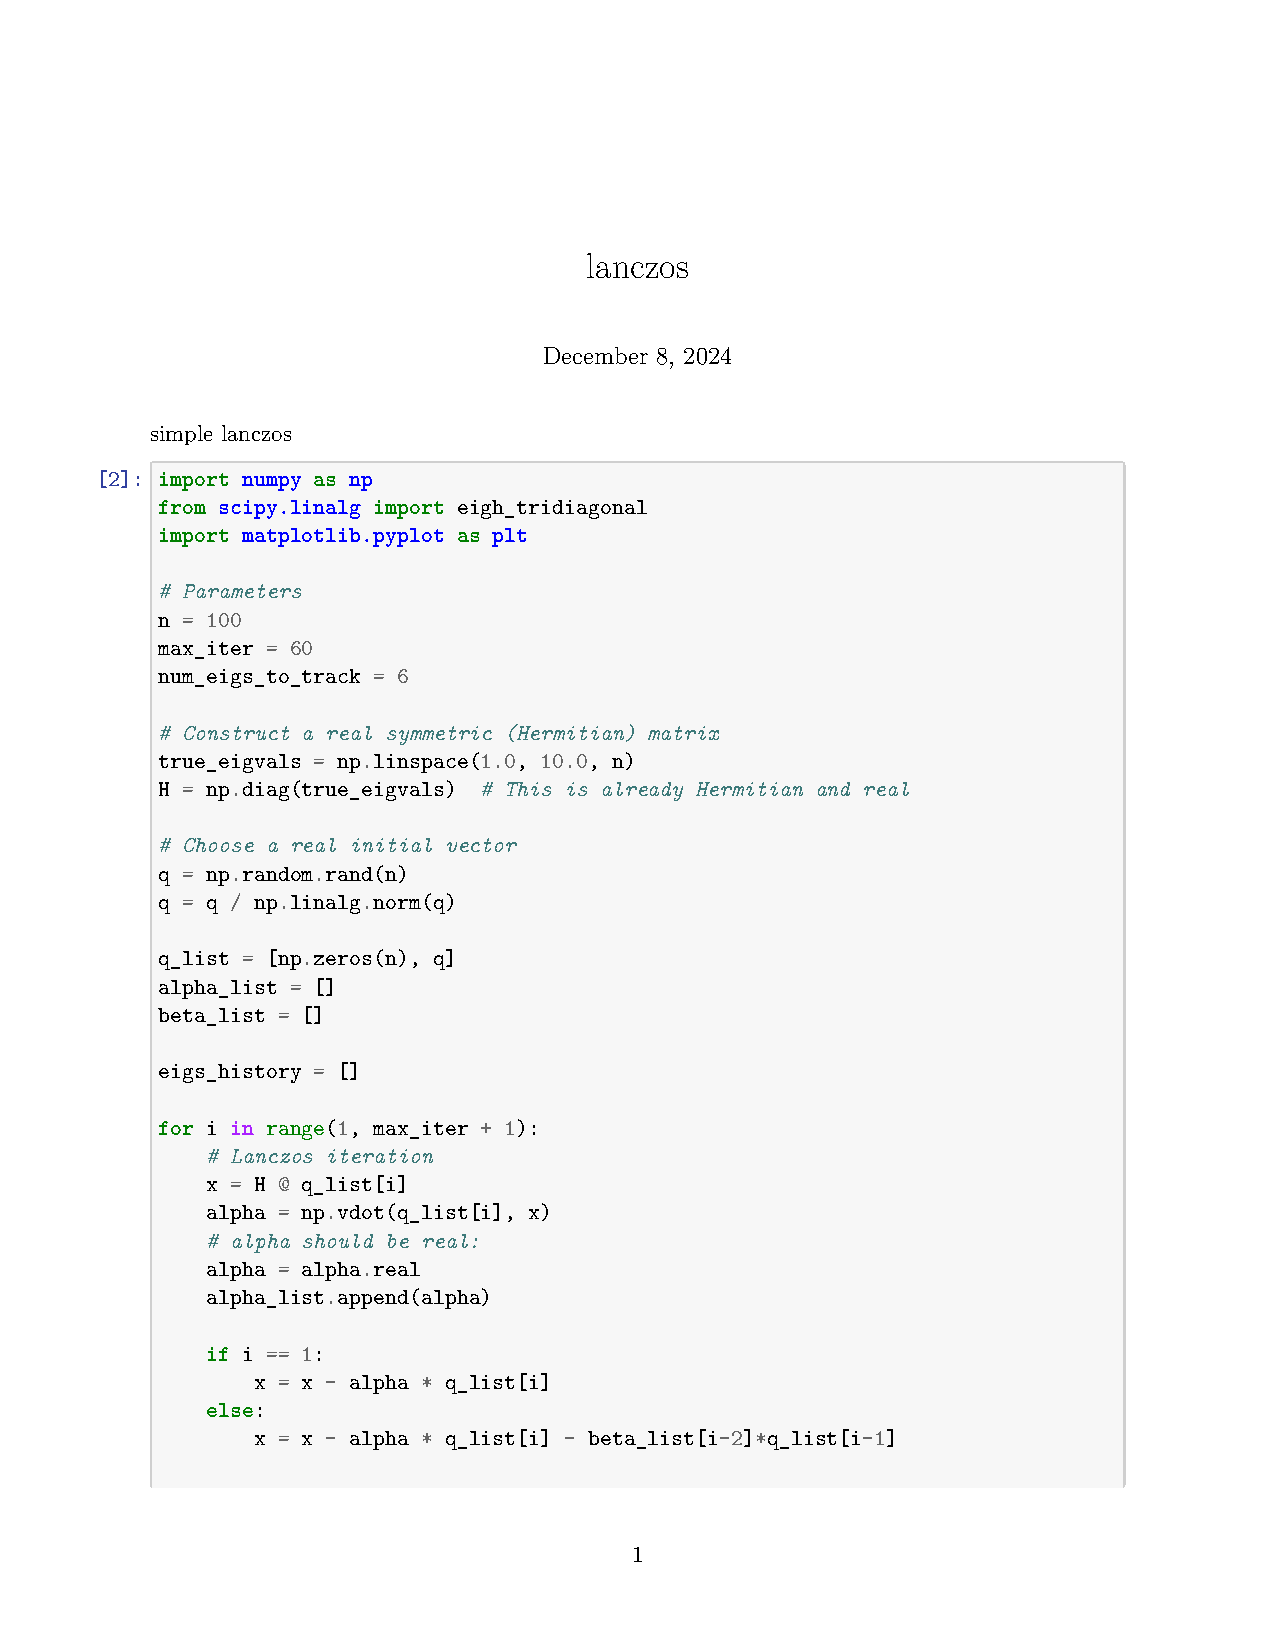
\includepdf[pages=-]{lanczos.pdf}
\end{document}
